\section{Lower Limb Weakness and Rehabilitation}
\subsection{Introduction}
Rehabilitation robotics systems are now used to treat different conditions. 
Two prominent conditions are spinal cord injuries (SCI) and strokes. While SCI and strokes are different medical conditions, they are highly traumatic to the body and cause motor damage to one or all limbs depending on the severity of the injury and the response of emergency intervention. Similar rehabilitation methods and robotic tools are currently being examined as a treatment for both injuries.  


\subsection{Spinal Cord Injuries}
In the United States, approximately 282,000 people are living with Spinal Cord Injuries (SCI), with approximately 17,000 new cases each year \cite{national2016facts}. SCI results in loss of motor function and sensor function. The amount of loss functionality depends on the injury level. As the injury location goes up the spinal cord, more functionality is lost, as shown in \autoref{fig:SCILevels}. The injury levels defined by the  American Spinal Injury Association (ASIA)  scale is as follows A–B; cervical (C7–C8) or thoracic (T1–T12) according to ASIA guidelines \cite{kirshblum2011international}. Accordingly, injuries level between C7-T12 are identified as the target requirement for lower limb exoskeleton studies \cite{esquenazi2012rewalk}. 

The injury level results in one of many classifications that define their functional ability. Paraplegia results in impairment of the trunk, legs, and pelvis. Tetraplegia results in the upper and lower body's impairment, including the arms, trunk, and other organs. An incomplete SCI is when there is some remaining sensory or motor function below the injury level.  Incomplete injuries, there is no motor or sensory functionality below the injury level. 

The cost of lifetime treatment is between \$500k -\$2M depending on the injury level \cite{mcdonald2002spinal}. This cost includes the initial cost immediately after the injury and the treatment of secondary health side effects.  

 

\begin{figure}
    \centering
    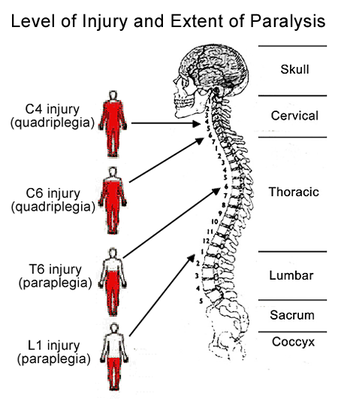
\includegraphics[scale=0.6]{images/background/SCI.png}
    \caption[Levels of SCI]{Levels of SCI \cite{sadaka2012bradycardia}}
    \label{fig:SCILevels}
\end{figure}

A secondary health side effect is a physical or psychological health condition caused by the disability \cite{jensen2012secondary}.  These side effects include the decrease in the bone density of the femur, decrease in blood pressure, and reduced muscle mass \cite{haisma2007complications} \cite{hitzig2010understanding}. These side effects result in a significantly reduced Quality of Life (QoL) of the person.  	\cite{craven2012impact}. Prevention of these side effects through rehabilitation will help increase the QoL and overall health of the person.  




\subsection{Strokes}
Strokes are a global health crisis with approximately 800,000 occurrences each year in the United States and is a leading cause of death worldwide \cite{george2017cdc} \cite{murphy2020stroke} \cite{feigin2015update}. While strokes have been decreasing worldwide, the rate of stroke in younger people (18-54 years old) has risen. The expected cause is increased hypertension, diabetes, lipid disorders, obesity, and tobacco use. 

A stroke is a medical condition where the blood vessels to the brain get blocked or burst; this means that the brain cannot get the necessary blood flow, and the tissue begins to die. There are broadly two different types of strokes \cite{perna2015rehabilitation}; ischemic strokes and hemorrhagic strokes as shown in \autoref{fig:strokes}. An ischemic stroke is caused by obstructed blood vessels. This type of stroke accounts for approximately 85\% of all strokes. A hemorrhagic stroke is caused when the blood vessels of the brain burst.  

\begin{figure}
    \centering
    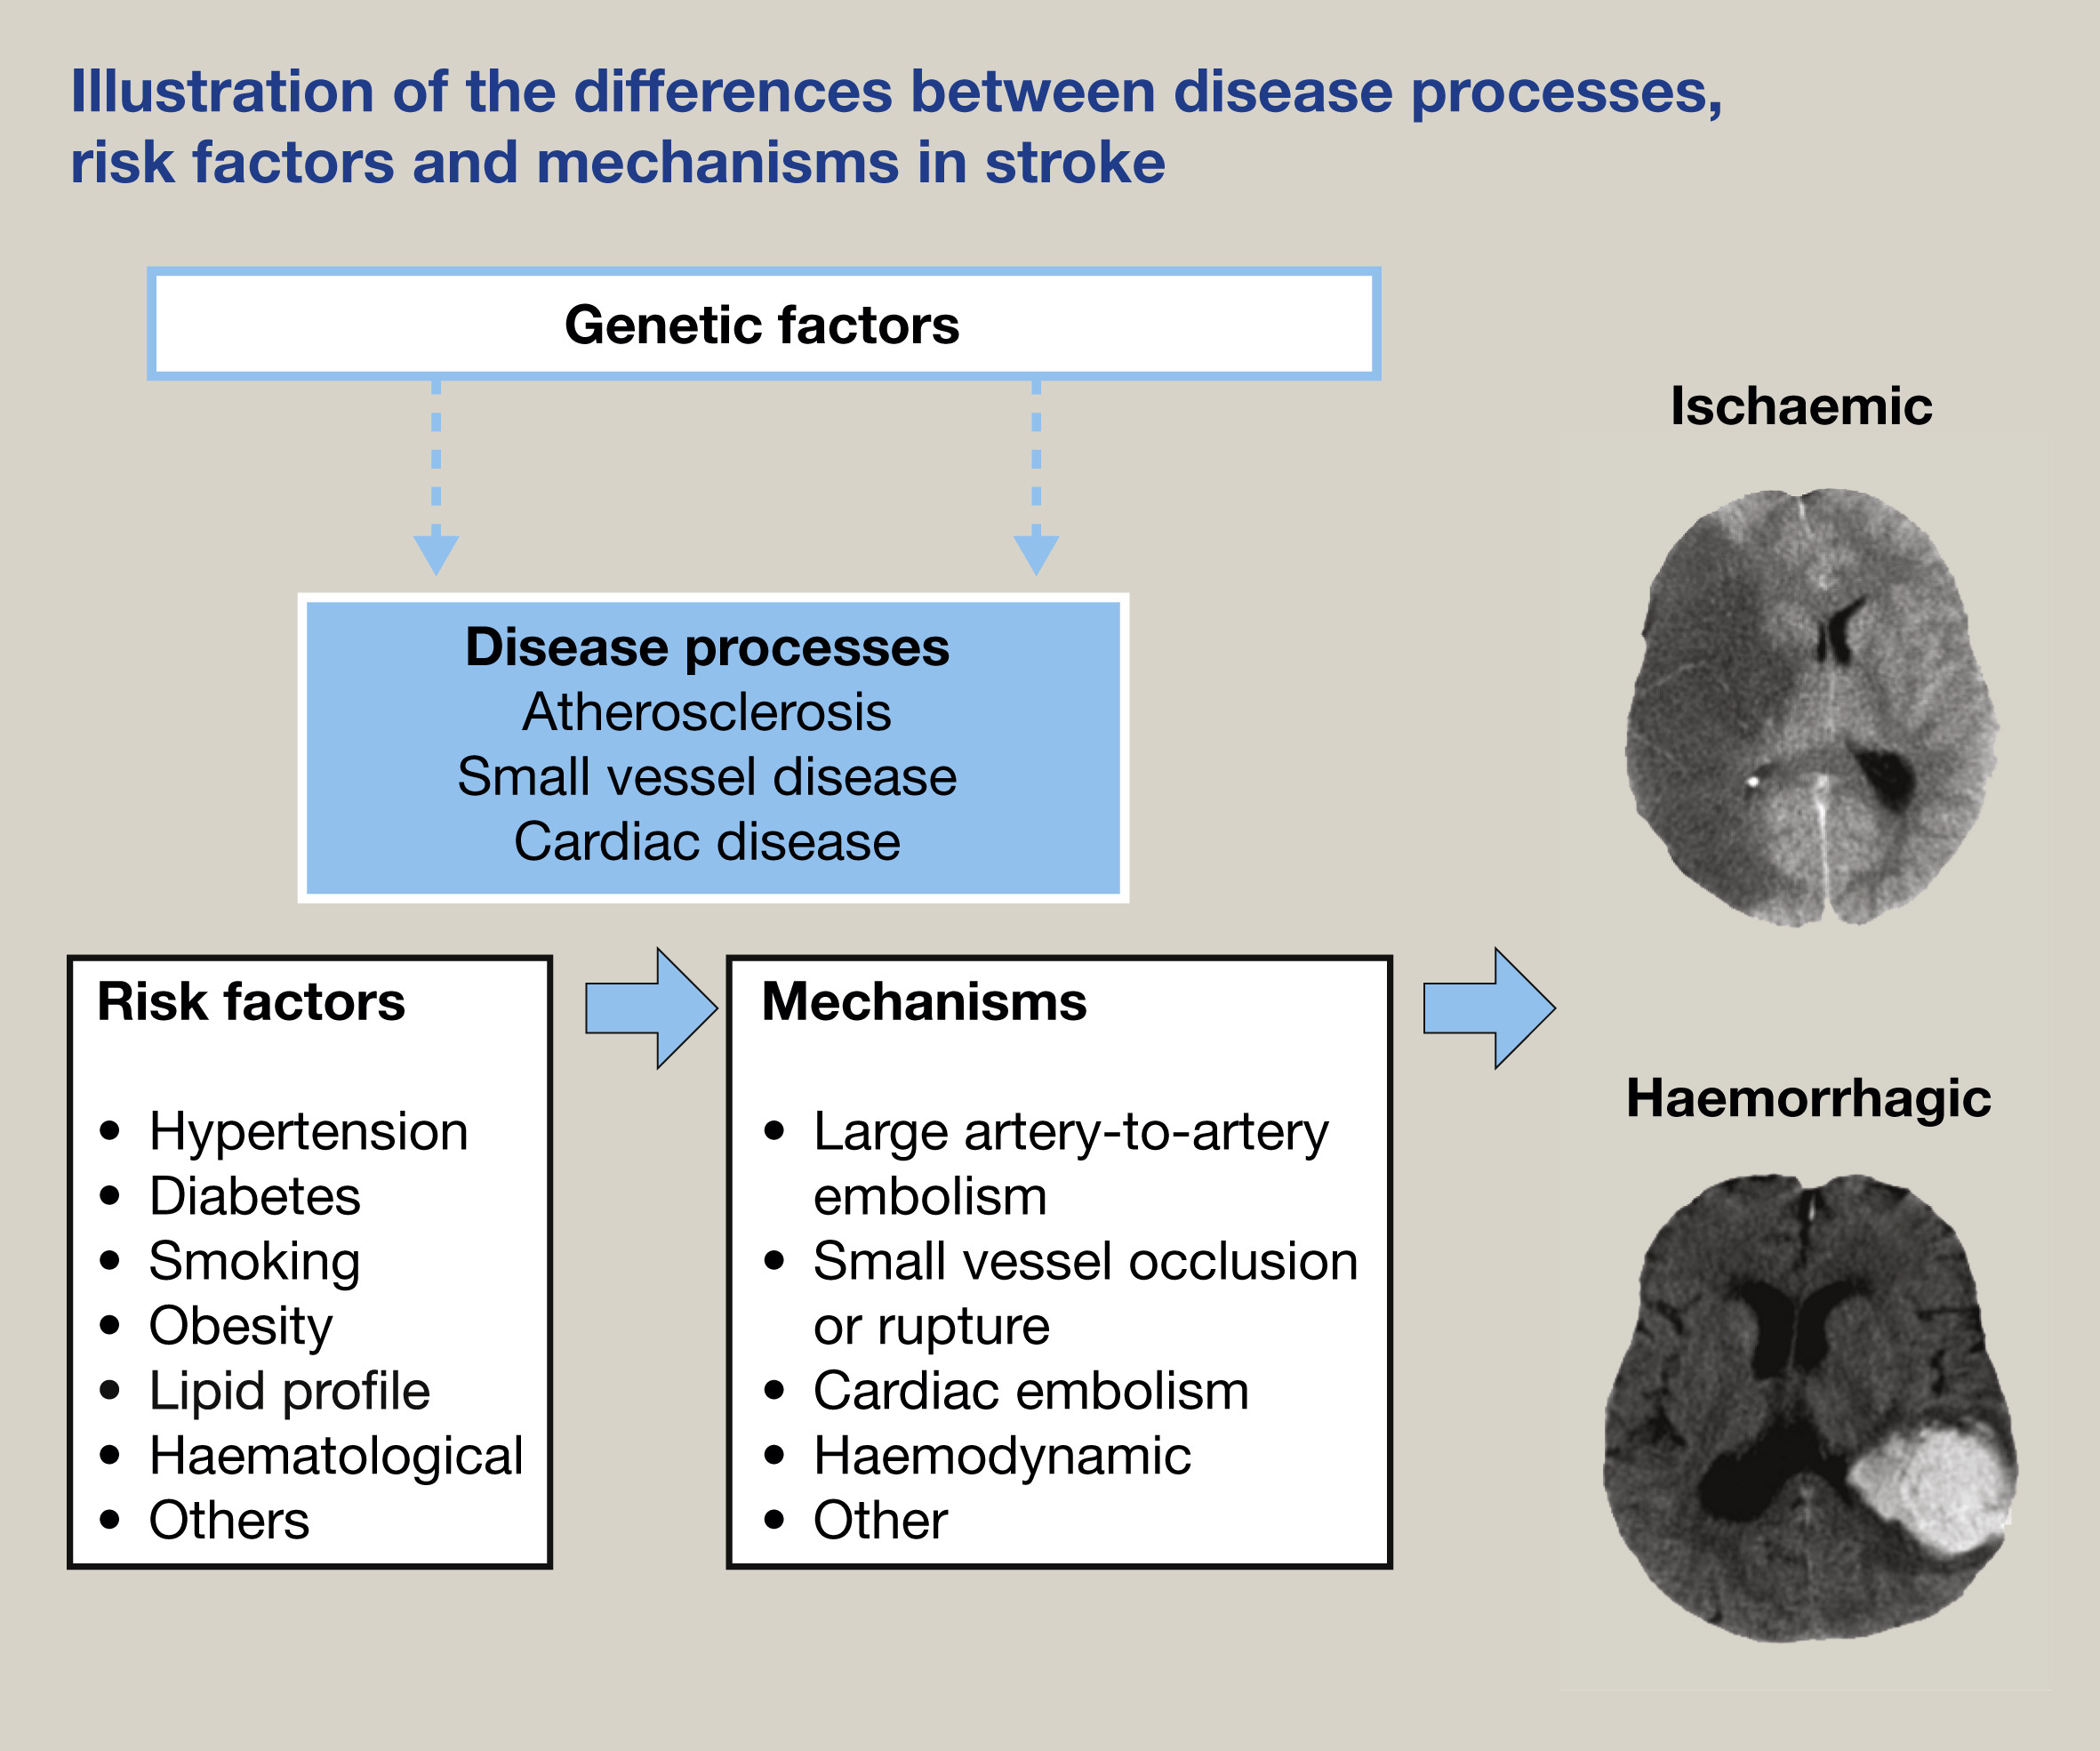
\includegraphics[scale=0.85]{images/background/stroke.jpg}
    \caption[Ischemic strokes and Hemorrhagic strokes]{Ischemic strokes and Hemorrhagic strokes \cite{murphy2020stroke}}
    \label{fig:strokes}
\end{figure}


It is crucial to receive treatment immediately after a stroke. Each minute causes more tissue and brain damage to occur \cite{saver2006time} resulting in about 1.9 million neurons per minute; this can result in both upper and lower limb weakness along with other cognitive complications \cite{pennycott2012towards}. Emergency treatment to restore blood flow has been shown to improve outcomes which are essential for getting the patient back to normal life with less loss of functionality \cite{goyal2016endovascular}.  



\subsection{Rehabilitation}
\label{sec:rehab}

 Rehabilitation is critical for regaining lost functionality and gaining independence to live a long, fruitful life; this does not mean that motor and sensory functionality will be completely or partially recovered but to reduce other medical side effects, have the ability to navigate the world and complete daily living activities (ADL), and improve QoL. QoL includes the betterment of the mental and emotional state of mind while mitigating the injury's physical side effects. By increasing the physical ability through physical rehabilitation and exercises, the person's QoL is improved \cite{noreau1995spinal}. Successful rehabilitation should teach a person how to physically navigate the world and give the person the motivation to interact with their community \cite{hammell2013spinal}.
 
 
 The rehabilitation process should start immediately after a traumatic injury. Most of the recovery progress is within the first year after the injury; this has been shown to have better long-term outcomes than delayed therapy \cite{scivoletto2005early} \cite{piepmeier1988late}.  The constraints of the wheelchair cause numerous long-term health problems. Being confined to a seat all day causes the leg muscle to atrophy \cite{castro1999influence}, the leg bones become weak \cite{goemaere1994bone} without a gravitational load, and get pressure sores \cite{wall2000preventing}. The complications lead to significant discomfort for the person and can lead to bone fractures and heart problems \cite{giangregorio2006bone}.  
 
 The primary cause of these health side effects can be prevented by exercise and loading the leg bones. Functional Electrical Stimulation (FES) is a rehabilitation tool used to stimulate muscle activation  \cite{quintero2012preliminary}. There are several benefits of using FES for SCI rehabilitation; clinical outcomes, fitness benefits, and functional gains \cite{hamid2008role}. FES has been used to allow people to stand, walk, and use a cycle\cite{mazzoleni2013fes}. All of which have measurable rehabilitation and health benefits. FES's main complication and limitation is muscle fatigue \cite{karu1995reducing}. Only using FES  does not provide any structural support to hold up the person. FES can be supplemented by using mechanical structures to support the patient and add a layer of safety. 
 
A mechanical orthosis helps the patient stand upright and walk and reduce and reverse some of these side effects \cite{palermo2017clinician}. The first systems were simple mechanical devices that assisted in ambulatory management, including Knee-Ankle-Foot-Orthosis (KAFO) or hip-KAFO (HKAFO). These devices performed poorly and required high metabolic energy expenditure \cite{del2012review}. As technology increased, these devices were made active using robotic technology, decreasing the patient's demand. These devices are discussed further in \autoref{sec:ExoBack}. The combination of FES and an active exoskeleton is called a hybrid exoskeleton \cite{ha2012enhancing} \cite{alouane2019hybrid}. 

Robotic exoskeleton-based rehabilitation does not necessarily produce better functional outcomes than traditional rehabilitation. However, one of the benefits of robotic rehabilitation is that it reduces the load on the therapist. Robotic exoskeletons can offer gait and balance training which is more than a single therapist might offer \cite{guidingLeg}, both the patient and the therapist reap the benefits. The patient receives gait training that follows an exact and repeatable motion, reducing the physical demand on the therapist, allowing them to focus more on patients and create more personalized care.  


A great deal of research has been published on the rehabilitation benefits of robotic rehabilitation. It has been used for post-SCI rehabilitation and post-stroke rehabilitation. For SCI, lower limb exoskeletons have had a significant focus in recent years, with several studies conducted \cite{esquenazi2012rewalk} \cite{zeilig2012safety} \cite{6876184}. Similar studies were conducted for stroke rehabilitation; however, it should be noted that upper arm exoskeletons have also been examined \cite{chang2013robot} \cite{ho2011emg}. 

The most common tests and metrics with robotic lower limb exoskeletons are; 6-minute walk test (6MWT) and the 10-meter walk test (10MWT) \cite{amatachaya2014concurrent}. Research has shown improvements in all the measured criteria. In general, increased walking velocity, walking distance, and endurance. The amount of improvement varied from subject to subject and was dependant on many factors, including injury level.   